%!TEX root = paper.tex
%%%%%%%%%%%%%%%%%%%%%%%%%%%%%%%%%%%%%%%%%%%%%%%%%%%%%%%%%%%%%%%%%%%%%%%%%%%%%%%%
\section{Background}
\label{sec:background}


%%%%%%%%%%%%%%%%%%%%%%%%%%%%%%%%%%%%%%%%%%%%%%%%%%%%%%%%%%%%%%%%%%%%%%%%%%%%%%%%
\subsection{Measurement Approaches}
\label{sec:measurementapproaches}

With these metrics, test parameters, and categorizations in mind, one can now attempt to conduct the actual measurements of which there are three distinct methods each situated at a unique vantage point as depicted in Fig.~\ref{fig:measurement-methods}.

\begin{figure}[!t]
    \centering
    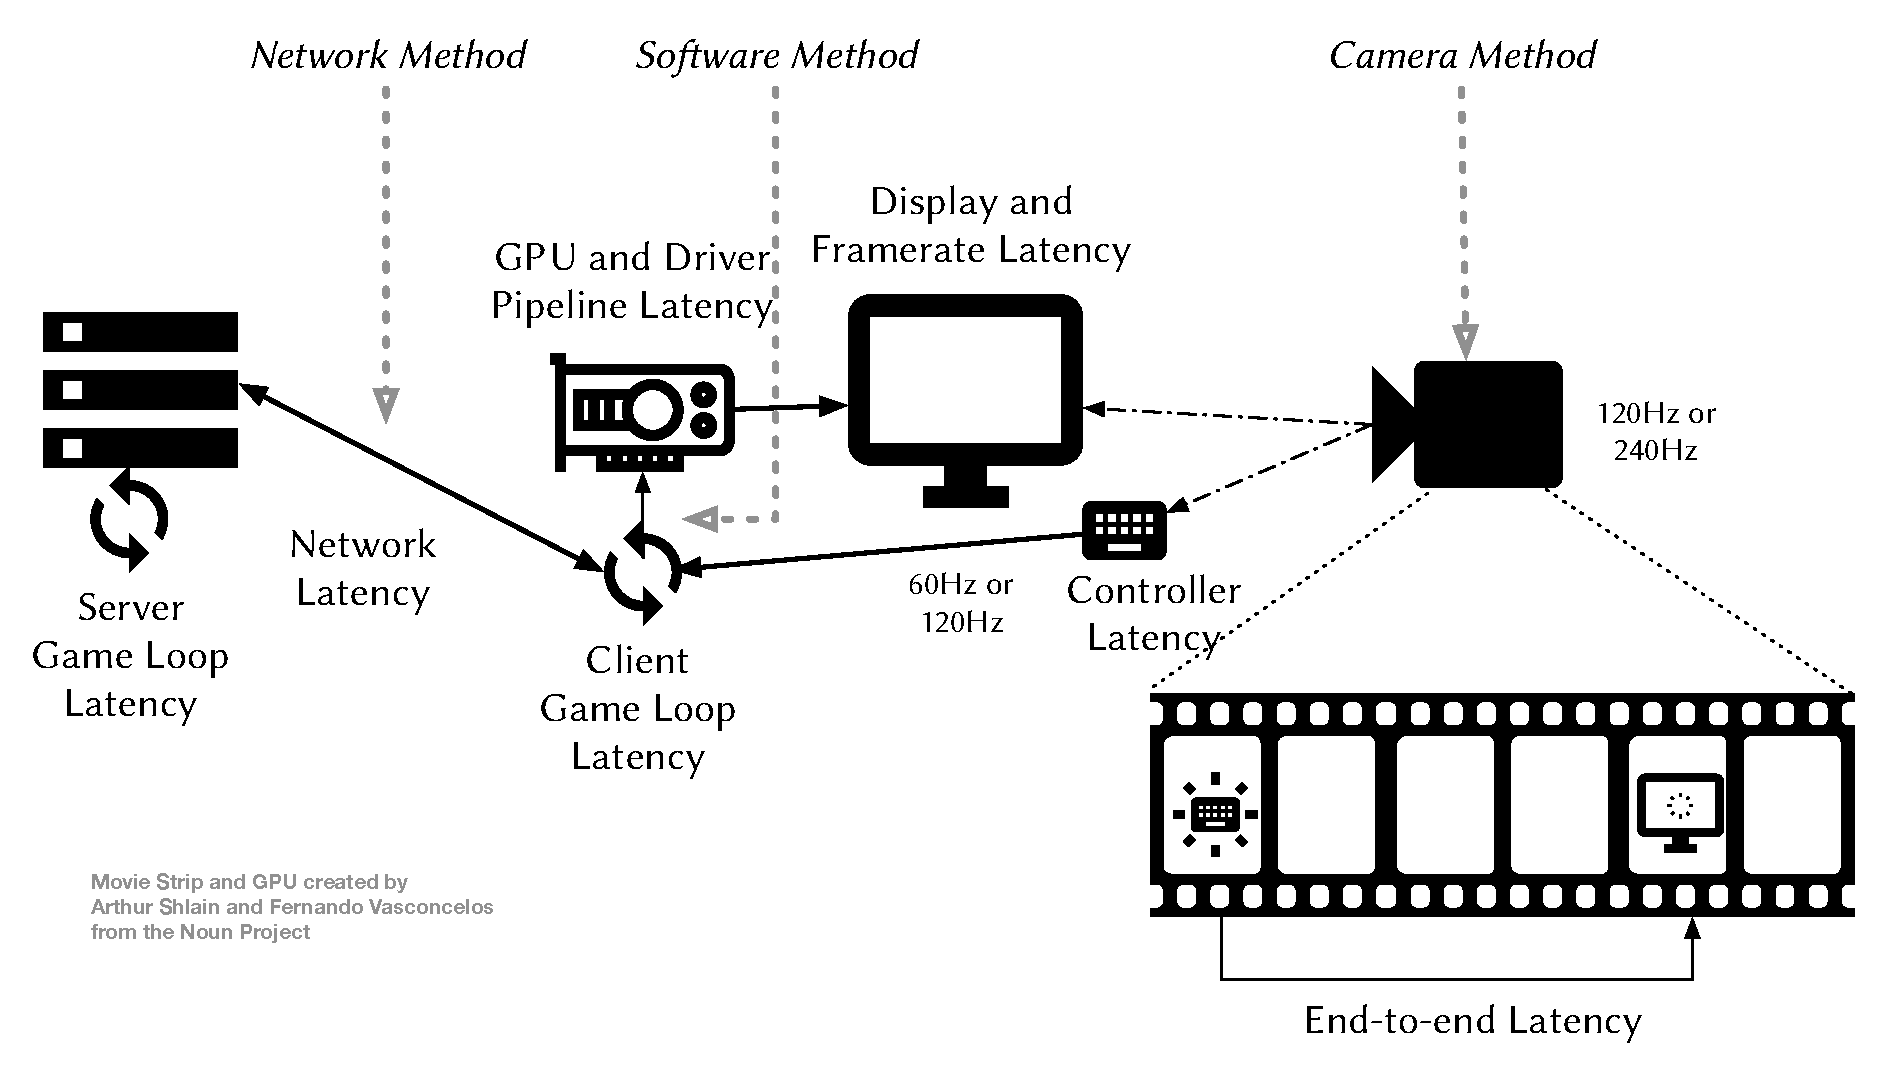
\includegraphics[width=1.0\columnwidth]{../models/e2e-lag.pdf}
    \caption{Location of the three measurement approaches to capture end-to-end latency inside a usual online video game lag chain.}
\label{fig:measurement-methods}
\end{figure}


%%%%%%%%%%%%%%%%%%%%%%%%%%%%%%%%%%%%%%%%%%%%%%%%%%%%%%%%%%%%%%%%%%%%%%%%%%%%%%%%
\subsubsection{Screen Recording Software Method}

Recording the output stream of a video game might be the simplest approach. It can capture both the framerate and \gls{IAT} at a driver level, and the recorded video can be used for image and quality analyses as well as to correlate it to additionally recorded input events to calculate the lag. This is not the the complete end-to-end lag however, as both the controller and screen output latency are missing. The need to install additional software might make it unsuitable for some scenarios, e.g., when measuring console video games. As a variant of this method, one can also record the output stream with a video capture card on a secondary computer, which does not negatively effect the game's performance as the software method does.

Examples of this approach include both \cite{Chen:2011:MLC:2072298.2071991} and \cite{6670099} which measured the end-to-end latency of cloud gaming services in the game client. They do this by invoking the system menu in games and measuring the time until it is displayed. A 2013 paper \cite{6574660} investigates the quality of cloud gaming interactiveness (i.e., the lag) as well as image quality by employing software recording methods on the client's computer.
%However, this method assumes a constant delay of game actions and may not capture the actual end-to-end lag of many of real game actions, as they are typically different from and longer as the latency of displaying a menu. A 2013 paper \cite{6574660} investigates the quality of cloud gaming interactiveness (latency) as well as image quality by employing software recording methods on the client's computer. With these techniques the challenges regarding the quality are discussed.


%%%%%%%%%%%%%%%%%%%%%%%%%%%%%%%%%%%%%%%%%%%%%%%%%%%%%%%%%%%%%%%%%%%%%%%%%%%%%%%%
\subsubsection{Passive Network Measurements}

In some cases it may also be advantageous to tap into the network interactions of the games and record the command and update messages sent between server and clients. While this is not a direct measure of game quality, it can give insights into the game's inner workings, such as the tick rates, and one can derive, e.g., the lowest achievable end-to-end lag from this.

%Can only investigate command and update messages, not tick rate directly. Evaluate rate, IAT, and bandwidth, estimate latency (though there may be no direct link between commands and updates).

Besides simple flow-based or packet-counting network metrics, many games also allow for deeper packet-dissecting analyses, as the often rely on standardized protocols or data formats, such as Protobuf\footnote{\url{https://developers.google.com/protocol-buffers/}} or incorporate well-known third-party multiplayer-enabling libraries. %And cloud games sometimes use derivates from the RTP-family or XMPP-based(VERIFY) protocols. 
Additionally, almost no game encrypts its time-critical messages, enabling an easy read-out. Through these means, the specific commands can be read from the network and potentially linked to their effect on the game state in the corresponding state update messages.
%, but also potentially allowing malicious actions to be taken easily.


%%%%%%%%%%%%%%%%%%%%%%%%%%%%%%%%%%%%%%%%%%%%%%%%%%%%%%%%%%%%%%%%%%%%%%%%%%%%%%%%
\subsubsection{Camera Recordings}

The only method to fully capture the end-to-end lag is to simultaneously record both the screen and input device through an external camera. The experimenter then has to count the frames between pressing a button on the input device and the action appearing on the screen and calculate the lag from this. For better visibility the input device is usually modified with an LED that turns on when the button is pressed. Also, the camera should operate at least at twice the monitor's refresh rate according to the Nyquist-Shannon sampling theorem. An additional benefit of this method is, that the game and the computers remain unaltered and are therefore not affecting any game mechanics. This approach is often used in the gaming press and by game developers to evaluate a game's control fidelity. A variant of this approach, replacing the camera with a photodiode and synthetically creating the input events with a microcontroller is described in \cite{beyermethod}, though it may be difficult to use for certain game actions that have a barely visible or unpredictable on-screen effect.



%%%%%%%%%%%%%%%%%%%%%%%%%%%%%%%%%%%%%%%%%%%%%%%%%%%%%%%%%%%%%%%%%%%%%%%%%%%%%%%%
\subsection{Related Work}
\label{sec:relatedwork}

Video game measurements have been a topic in many past papers. Due to the strong interactivity of games and the large number of different game mechanics many papers focus on conducting user studies and simply note the subjective quality of the users. But the outcome of these studies still depends very much, e.g., on the precise setup, the game, and the selection of players. The following represent a few examples of such studies. 

In \cite{5976180} Jarschel et al. identify some influence factors on the subjective quality of cloud gaming through a user survey for certain games and three different game categories (slow, medium, fast games) that have been subjected to worsening \gls{QoS} parameters. Downstream packet loss and delay was noted be be especially problematic for achieving a good quality. Similarly, the authors \cite{4591393} observed the relationship of players quitting a \gls{MMO} game with deteriorating \gls{QoS} and noted an impact proportion of 1:2:4:3 for delay, jitter, and packet loss on both the client-to-server and server-to-client connections respectively. Additionally, a user study in \cite{4604397} also showed a correlation of the \gls{MOS} to the delay as well as the jitter for another \gls{MMO}, in this case the total delay had more impact than the delay variation. Regarding the subjective quality in first person shooters, the authors of \cite{6614351} find a strong impact of the delay and packet loss on the experienced quality. The authors of \cite{6404025} and \cite{beyerusing} use \gls{fEMG} and \gls{EEG} approaches respectively to examine individual gamers' reaction to various cloud games and measure the quality they are experiencing in terms of real-time strictness and \gls{MOS}. Finally, an ITU-T Recommendation \cite{mollertowards} concerning subjectively measuring video game \gls{QoE} is also in preparation, which discusses game-relevant \gls{QoS}-metrics as well as the selection of players and games.

In order to avoid some of the issues with subjective user studies other approaches examine the players' objective performance through in-game metrics such as the game's highscore or the duration to achieve a certain task. For example, a user study \cite{Chen:2006:SOG:1167838.1167859} observers in another \gls{MMO} a decrease in the objective quality assessment metrics (the playing duration) due to the influence of network \gls{QoS} (higher delay, delay variation, as well as loss). A 2006 paper \cite{Claypool:2006:LPA:1167838.1167860} categorizes player actions and their relationship to latency, with special regards for the actions' precision as well as their deadline. However, the in-game metrics under study can not represent short-term effects of latency as they operate on much larger time-scales. 
%(e.g. researching the whole technology tree in Warcraft 3 is neither a representative action of the game nor delay-sensitive at all). Also the presence of lag compensation techniques is not considered. The end result is a delay tolerance table which probably is not very representative of modern video games.
A second paper by Claypool et al. \cite{claypool2007} furthers this notion of the influence of network \gls{QoS} on in-game actions and specifically looks at players' performance in first person games. A user study records the performance in artificially created in-game environments. Here, the performance gets worse with a degraded network, but at a very slow pace. %Players were also subjected to very low framerates of \SI{7}{\hertz} and \SI{3}{\hertz}, which is such an unrealistic setting, that it should not even have been tested. The reasons for this are laid out in Section~\ref{sec:framerate}.
\cite{1266180} investigates the kills per minute in the first person shooter \textsc{Quake 3} and sees a steady decline of this performance metric with increasing network delay to real live game servers. However, another paper \cite{Beigbeder:2004:ELL:1016540.1016556}, looking at player performance in \textsc{Unreal Tournament 2003} in a controlled in-game environment, finds almost no influence of increased delay and packet loss, even at high values of \SI{200}{\milli\second}. %The discrepancy between the otherwise similar studies could potentially be attributed to the specific construction of the in-game test environment. 
A 2002 paper \cite{Pantel:2002:IDR:507670.507674} which gathered objective \gls{QoE} measurements from a custom-made RC racing video game again sees a strong dependence of the player's performance on the delay, and suggests that a network \acrshort{RTT} of \SI{200}{\milli\second} is barely usable and \SI{500}{\milli\second} completely unusable. Finally, the authors of \cite{Bredel:2010:MSR:1944796.1944797} also find a strong and negative influence of high delay on the player's performance, in this case again in \textsc{Quake 3}. 

It is interesting to note the discrepancies both in terms of the influencing parameters as well as their degree in between the studies. Considering the complexity and variability of video games and the difficulties of finding and setting up good comparable scenarios and testbeds, it is understandable that some studies come to different results. This makes it much more important to first understand the basic components of online video games and how they can interact. An appropriate experimental setup can be defined and data recorded in a more meaningful way with these components in mind.






%Pure \gls{QoS} views on the quality of online video games are rather are, but are nonetheless important in correctly assessing any game-related parameters and are also the foundation for most objective and subjective \gls{QoE} studies.



%A 2012 article notes the dependence of gaming on latency and the difficulties cloud-based solutions have in providing a sufficiently low latency. The suggest a move closer to the edge to reach more users in a quality they deem adequate.  \cite{Choy:2012:BSC:2501560.2501563}.
%``The Brewing Storm in Cloud Gaming: A Measurement Study on Cloud to End-user Latency'' 

%``Placing Virtual Machines to Optimize Cloud Gaming Experience'' \cite{6853364}  interesting for cloud gaming economics

%Adaptive Mobile Cloud Computing to Enable Rich Mobile Multimedia Applications \cite{6413270}

%Addressing Response Time and Video Quality in Remote Server Based Internet Mobile Gaming \cite{5506572} optimize mobile cloud gaming based on a certain impairment function and by reducing video bitrate and fps (even sub 10fps...)

%``Kahawai: High-Quality Mobile Gaming Using GPU Offload'' \cite{Cuervo:2015:KHM:2742647.2742657}

%``Outatime: Using Speculation to Enable Low-Latency Continuous Interaction for Mobile Cloud Gaming'' \cite{Lee:2015:OUS:2742647.2742656}

%``Assessing the Impact of Game Type, Display Size and Network Delay on Mobile Gaming QoE'' \cite{beyer2014typedisplaydelayimpact} Another user study regarding context factors like screen size and their impact on MOS, but also game type and delay on MOS

%A Method For Feedback Delay Measurement Using a Low-cost Arduino Microcontroller \cite{beyermethod} already covered in measurement methods section

%``QoE Assessment of Interactivity and Fairness in First Person Shooting with Group Synchronization Control'' \cite{Ida:2010:QAI:1944796.1944806} interessant für lag compensation betrachtungen

%``The Impact of Video Encoding Parameters and Game Type on QoE for Cloud Gaming: a Case Study using the Steam Platform'' \cite{slivarimpact}

%``How Do New Visual Immersive Systems Influence Gaming QoE?'' \cite{hupontnew} Vergleich Immersion am monitor vs oculus. beispiel eines schlechten testsetups, da unterschiedliche FoV für beide ausgabetypen (75° vs 100°), test wird stark verfälscht

%%``An experimental estimation of latency sensitivity in multiplayer Quake 3''  vs. \cite{1266180} ``The Effects of Loss and Latency on User Performance in Unreal Tournament 2003'' \cite{Beigbeder:2004:ELL:1016540.1016556}. both papers completely contradict each other: Quake 3: significant impact of latency on game performance (kills/minute); UT3: no impact on user performance at all (kills/deaths per game)

%``Security issues in online games'' \cite{doi:10.1108/02640470210424455}